% The ring Z[sqrt(2)] embedded as a lattice in R^2 via the two real
% embeddings a + b sqrt(2) |-> (a + b sqrt(2), a - b sqrt(2)), with the
% fundamental parallelepiped spanned by 1 and sqrt(2) shaded.
% Source: book/tex/alg-NT/classgrp.tex (§ The discriminant of a number
% field) — asy figure.
\documentclass[border=2mm]{standalone}
\usepackage{tikz}
\begin{document}
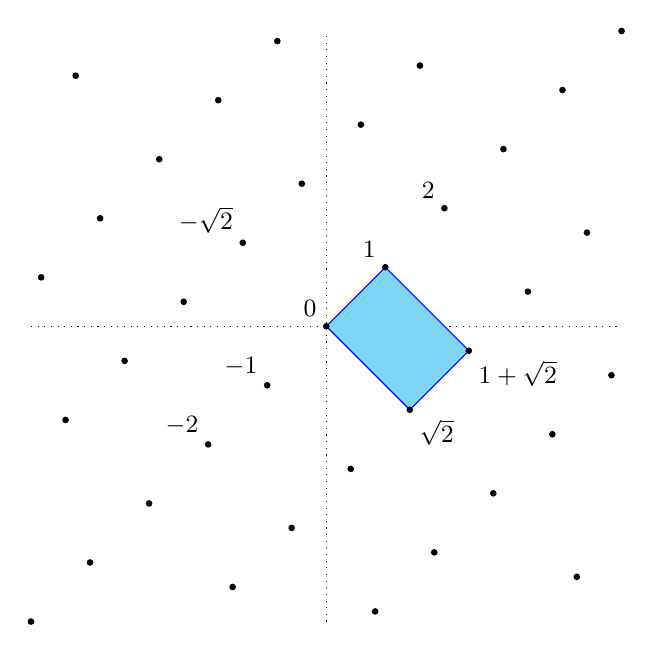
\begin{tikzpicture}[scale=0.75]
  \pgfmathsetmacro{\T}{sqrt(2)}
  \draw[dotted] (-5,0) -- (5,0);
  \draw[dotted] (0,-5) -- (0,5);
  \filldraw[fill=cyan!50, draw=blue]
    (0,0) -- (1,1) -- (1+\T,1-\T) -- (\T,-\T) -- cycle;
  \foreach \a in {-10,...,10}
    \foreach \b in {-10,...,10}
    {
      \pgfmathsetmacro{\px}{\a+\T*\b}
      \pgfmathsetmacro{\py}{\a-\T*\b}
      \pgfmathparse{abs(\px)<=5 && abs(\py)<=5 ? 1 : 0}
      \ifnum\pgfmathresult=1
        \fill (\px,\py) circle (1.6pt);
      \fi
    }
  \node[above left, font=\small] at (-2,-2) {$-2$};
  \node[above left, font=\small] at (-1,-1) {$-1$};
  \node[above left, font=\small] at (0,0) {$0$};
  \node[above left, font=\small] at (1,1) {$1$};
  \node[above left, font=\small] at (2,2) {$2$};
  \node[above left, font=\small] at (-\T,\T) {$-\sqrt 2$};
  \node[below right, font=\small] at (\T,-\T) {$\sqrt 2$};
  \node[below right, font=\small] at (1+\T,1-\T) {$1+\sqrt 2$};
\end{tikzpicture}
\end{document}
